\subsubsection{A Software Build Case Study}
\label{sec:build}

\begin{figure}[htbp]
\begin{center}
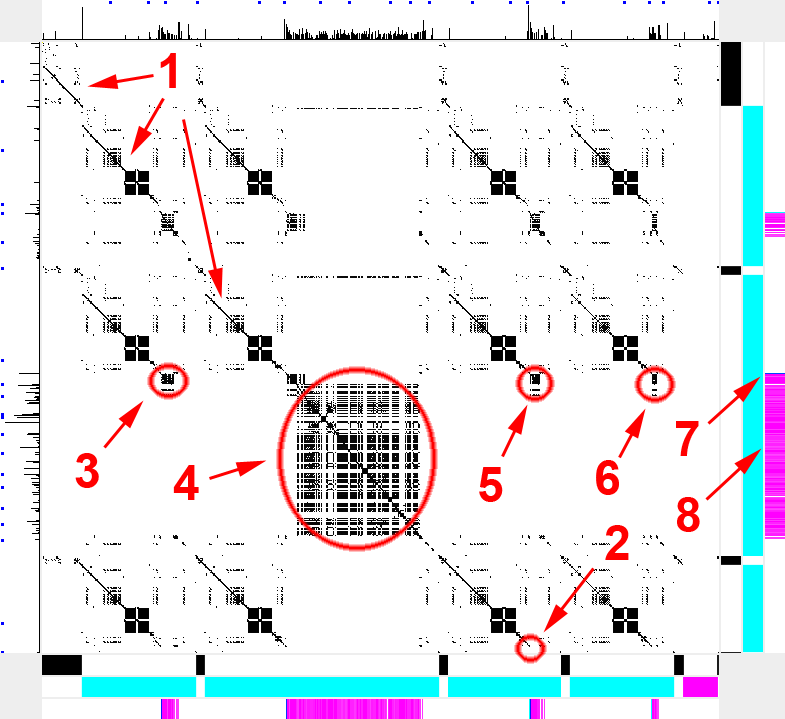
\includegraphics[width=0.8\columnwidth]{lviz/make-fail.png}
\caption{Event-ordered VDP comparing a successful (x-axis)
software build process and a failed (y-axis) one.
%DP matching: program, operation and value (pathname);
%DP color: any=black;
%Bar1: {\tt nmake.exe}=black;
%Bar2: {\tt cl.exe}=cyan, {\tt link.exe}=magenta;
%Bar3: reading {\tt .c}/{\tt .h} files = cyan/magenta.
\label{fig:make-fail}
}
\begin{tabular}{ll}
DP match : & program + operation + value (pathname)\\
DP color : & black $\rightarrow$ any\\
Bar1 color : & black $\rightarrow$ {\tt nmake.exe}\\
Bar2 color : & cyan $\rightarrow$ {\tt cl.exe}; magenta $\rightarrow$ {\tt link.exe}\\
Bar3 color : & cyan $\rightarrow$ reading {\tt .c} files;\\
 & magenta $\rightarrow$ reading {\tt .h} files
\end{tabular}
\end{center}
\end{figure}

\begin{figure}[htb]
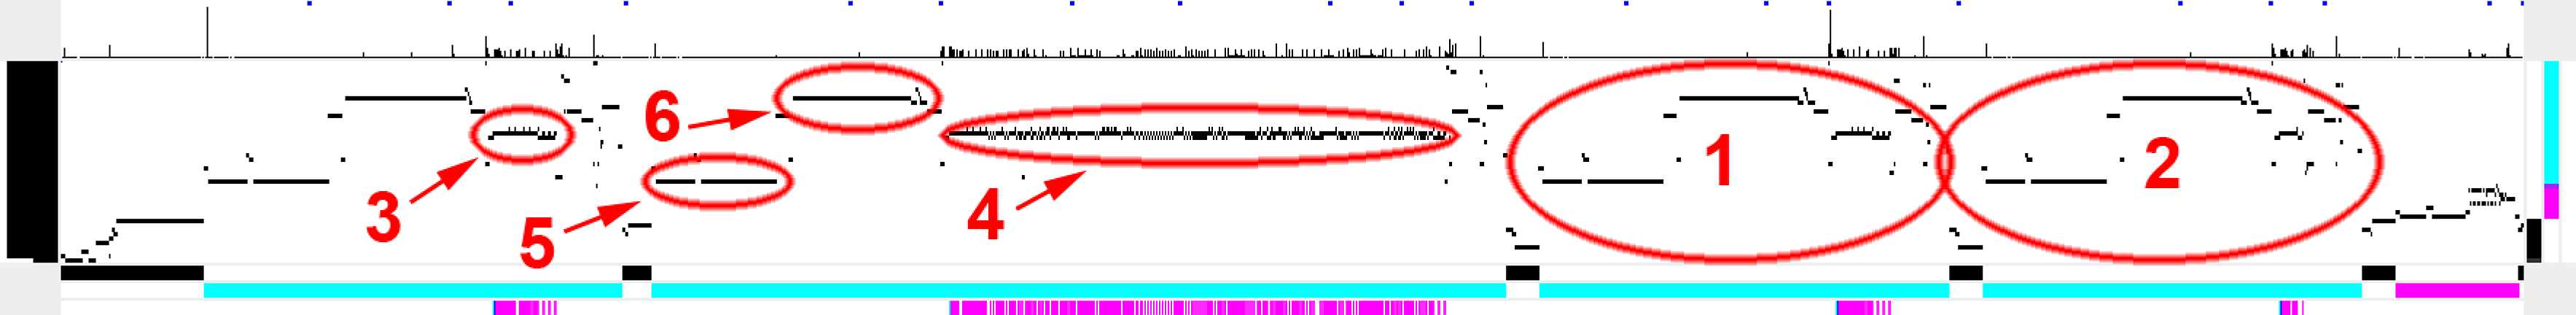
\includegraphics[width=1.0\textwidth]{lviz/make-pp.png}
\caption{Program point event-ordered VDP of project build: pseudo program point trace (y-axis).}
DP match: program name + program point;
DP color: black $\rightarrow$ any;
Barcode coloring rules are the same as in Figure~\ref{fig:make-fail};
Bar3 in y-axis is undefined as the pseudo trace does not have operation type.
\label{fig:make-pp}
\end{figure}

We now apply visualization to diagnose program failure.
In Figure~\ref{fig:make-fail}, we compare a successful software project build
with a failed one to explain the failure.
The project consists of 4 C files, a header file and a {\tt makefile}.
We use {\tt nmake.exe} from Visual Studio to build the project.
To deliberately cause failure, one of the C files is changed
to be unreadable.

% Before identifying the cause of the failure,
We first explain what the visualization shows.
From the Bar2 of x-axis, 
we can see 4 {\tt cl.exe} processes (4 cyan regions), which tallies
with the number of C files.
There is one invocation of {\tt link.exe} (magenta),
occurring at the end of the trace.
By correlating Bar2 and Bar3, we see that
{\tt cl.exe} processes first read a C file (tiny blue bar in region {\em 7})
and then read a number of header files (long magenta bar in region {\em 8}).
Different {\tt cl.exe} processes read a different number of header files,
see sizes of regions {\em 3}, {\em 4}, {\em 5}, {\em 6} differ.

In a self-comparison VDP, there will be a 45$^\circ$
diagonal line from top-left to bottom-right corner.
% The diagonal line means that the events
% on both x-axis and y-axis match (which is obviously true for self-comparison).
Figure~\ref{fig:make-fail} shows a 45$^\circ$ diagonal (Label {\em 1})
with some breaks, from
the start to region {\em 2}, near the end of the failed build (y-axis).
It shows that the traces are basically similar till the failure point
when the build terminates.
By zooming in (not shown),
we see that the failure occurs at the third invocation of
{\tt cl.exe}, just before reading the C file.
Thus, the VDP shows how file I/O works in the build and we use this
to identify a failed build.
One might argue that the compiler's error message is a better solution.
However, firstly,
not all software give detailed error message like the compiler in this case.
Secondly, due to software bugs, the error message could be wrong, while 
the system trace reports the actual underlying issues.

The build example is reused to show a visualization of the code structure
of {\tt cl.exe} in Figure~\ref{fig:make-pp}.
We use a pseudo trace (y-axis) consisting of the program name
concatenated with its program point in the binary (an instruction address)
which is sorted by program name and address.
The program point comes from the stack walk corresponding to the event
and corresponds to the latest return address in the stack trace
coming from the executable or earliest DLL.
The x-axis trace is as before in Figure~\ref{fig:make-fail}.

Region {\em 1} and {\em 2} show two invocations of {\tt cl.exe}
having similar patterns.
In fact, all 4 invocations follow the same pattern which can be broken
up into three main components:
region {\em 5}, {\em 6} and {\em 4}.
By zooming in and looking at the events, we infer that
region {\em 5} and {\em 6} is in the initialization phase of the compiler, which include
loading of DLL files and reading configurations from the registry.
Region {\em 6} is the reading of a large DLL {\tt rsaenh.dll}.
By looking at Bar3,
region {\em 3} and {\em 4} are the reading of C and header files.
As different C files have different header includes,
region {\em 3} and {\em 4} have different widths.
The fine squiggles in region {\em 3} and {\em 4} represent
three different file operations: open, read and close.
For each header file, there is one file open and close event,
with a differing number of file read operations depending
on the file size.
This makes the squiggles irregular.
Since this VDP is based on program points, it shows directly the 
structure of the function calls. Thus, it visualizes
the code while Figure~\ref{fig:make-fail} compares the operations
due to system calls.
It is also different from the source code
visualization~\cite{lefebvre2009tralfamadore} and we do not need to rely on
availability of source code.

The configurations play an important role in a VDP.
Figure~\ref{fig:make-matching} shows two VDPs
which are visually different from each other and also Figure~\ref{fig:make-fail}
but they are all visualizations of the same underlying trace.
The VDPs in Figure~\ref{fig:make-matching} and
Figure~\ref{fig:make-fail} only differ in the DP matching rule and
the rest of the configuration is the same.
% The rest of the configuration and the two traces are exactly the same.
The left side VDP in Figure~\ref{fig:make-matching} uses only the event
operation as the DP matching rule.
It can be used to highlight same or different operations.
The right side VDP uses the program name, and can be used to
show different programs used in the project build process.

\begin{figure}[htb]
\begin{center}
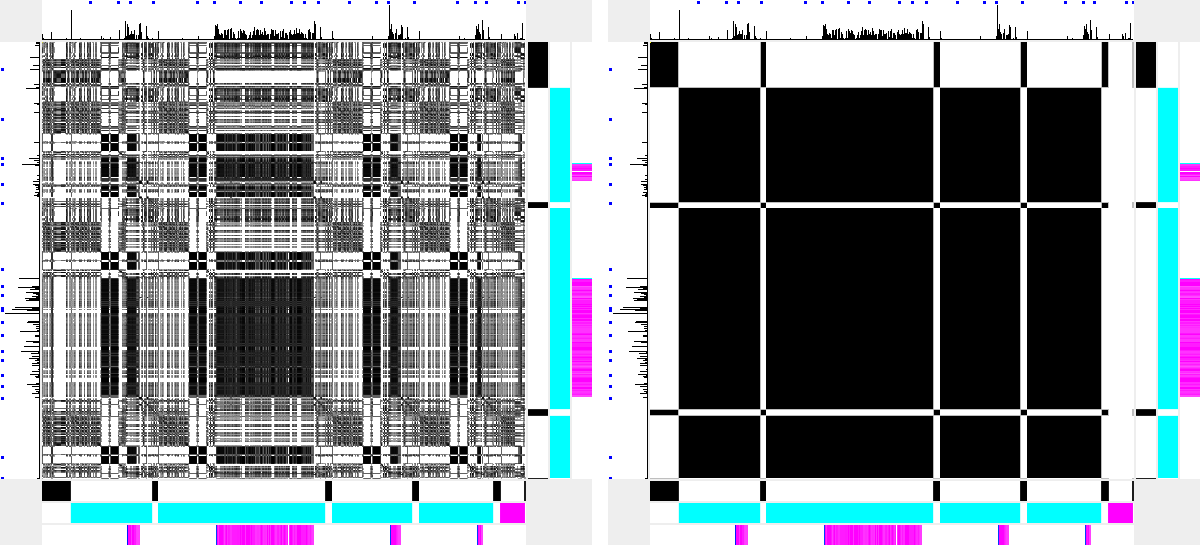
\includegraphics[width=1.0\columnwidth]{lviz/make-matching.png}
\caption{Changing the DP matching rule of Figure~\ref{fig:make-fail}.
Left side DP matching rule is operation; Right side is program name.
}
\label{fig:make-matching}
\end{center}
\end{figure}

% \TODO{reviewer 2:
% In the second example, figure 8, a similar question: how do I know that a cyan
% bar is cl.exe and not some other process - as a user I mean, not reading the
% legend of the figure? But the main question I have is why would a user go to
% this level of effort to find why a build failed, he can always use the
% compiler's build log to find much more precisely and more quickly what
% happened.  fixed.
% }
